\subsection{Home Page}

\begin{figure}[htbp]
  \centering
  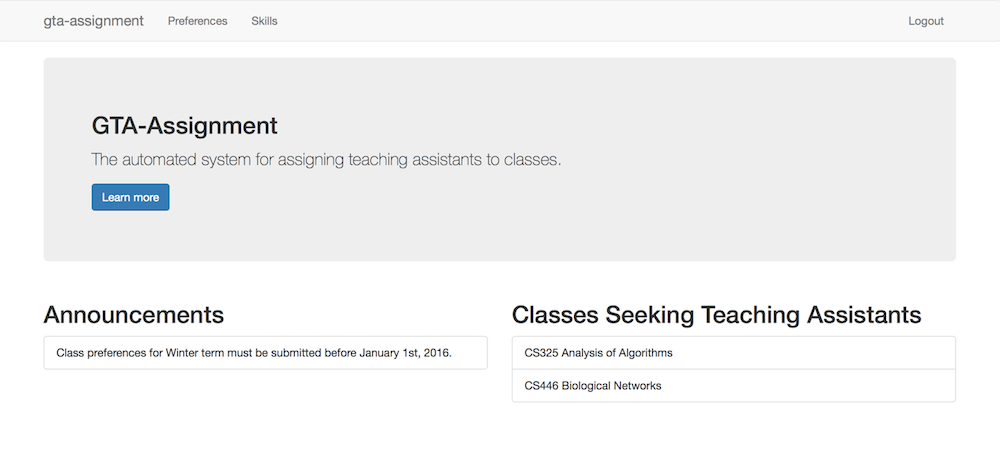
\includegraphics[width=0.75\linewidth]{images/homepage-design.png}
  \caption{Mock Homepage}
\end{figure}

\begin{figure}[htbp]
  \centering
  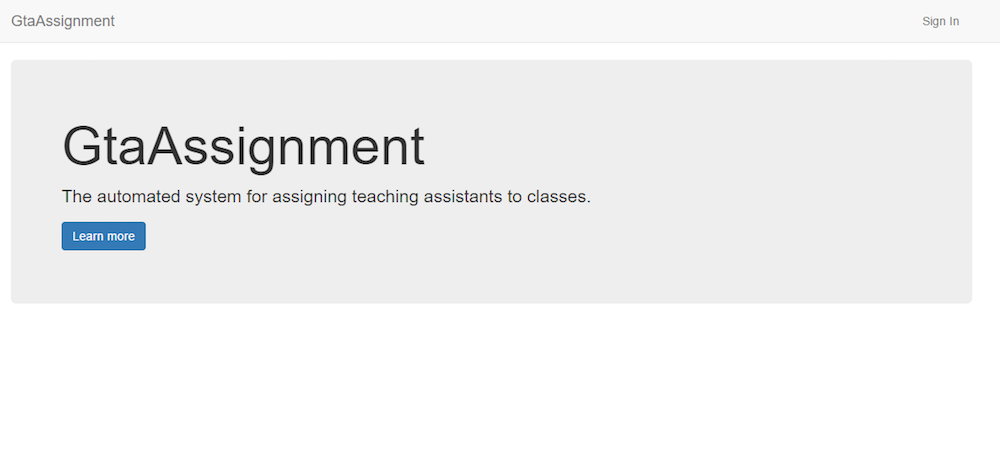
\includegraphics[width=0.75\linewidth]{images/homepage-alpha.png}
  \caption{Alpha Homepage}
\end{figure}

\begin{figure}[htbp]
  \centering
  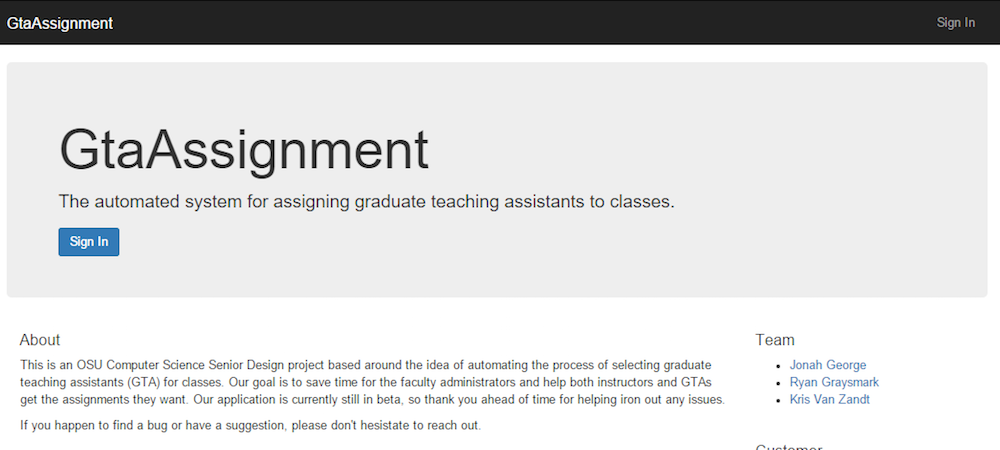
\includegraphics[width=0.75\linewidth]{images/homepage-beta.png}
  \caption{Release Homepage}
\end{figure}

Comparing what we had for our Alpha and what we have for Release, you can see that we fully wrote an 'About' and 'Learn More' section.
Those two sections have replaced the 'Announcements' and 'Classes Seeking Teaching Assistants' which we had from our design document.
These sections give a concise look into our project for anyone who has neveer seen or heard of the site before.
One can also see that at the top right we have the Sign In button, which is configured to log users in with Google OAuth2.
We have also been able to configure the integration to only grant access to users with a Oregon State ONID accounts.
